\section{Slice Layouts}
    \subsection{PIN Slice Layout}
        The PIN slice layout consists of 3 cells from the provided library.
        They were arranged as to provided maximum material density and
        uniformity among the power rails.  The connections in and out of the
        slice are arranged such that slices can be directly patterned together
        with little to no additional connections at a higher level.
        \begin{figure}[H]
            \centering
            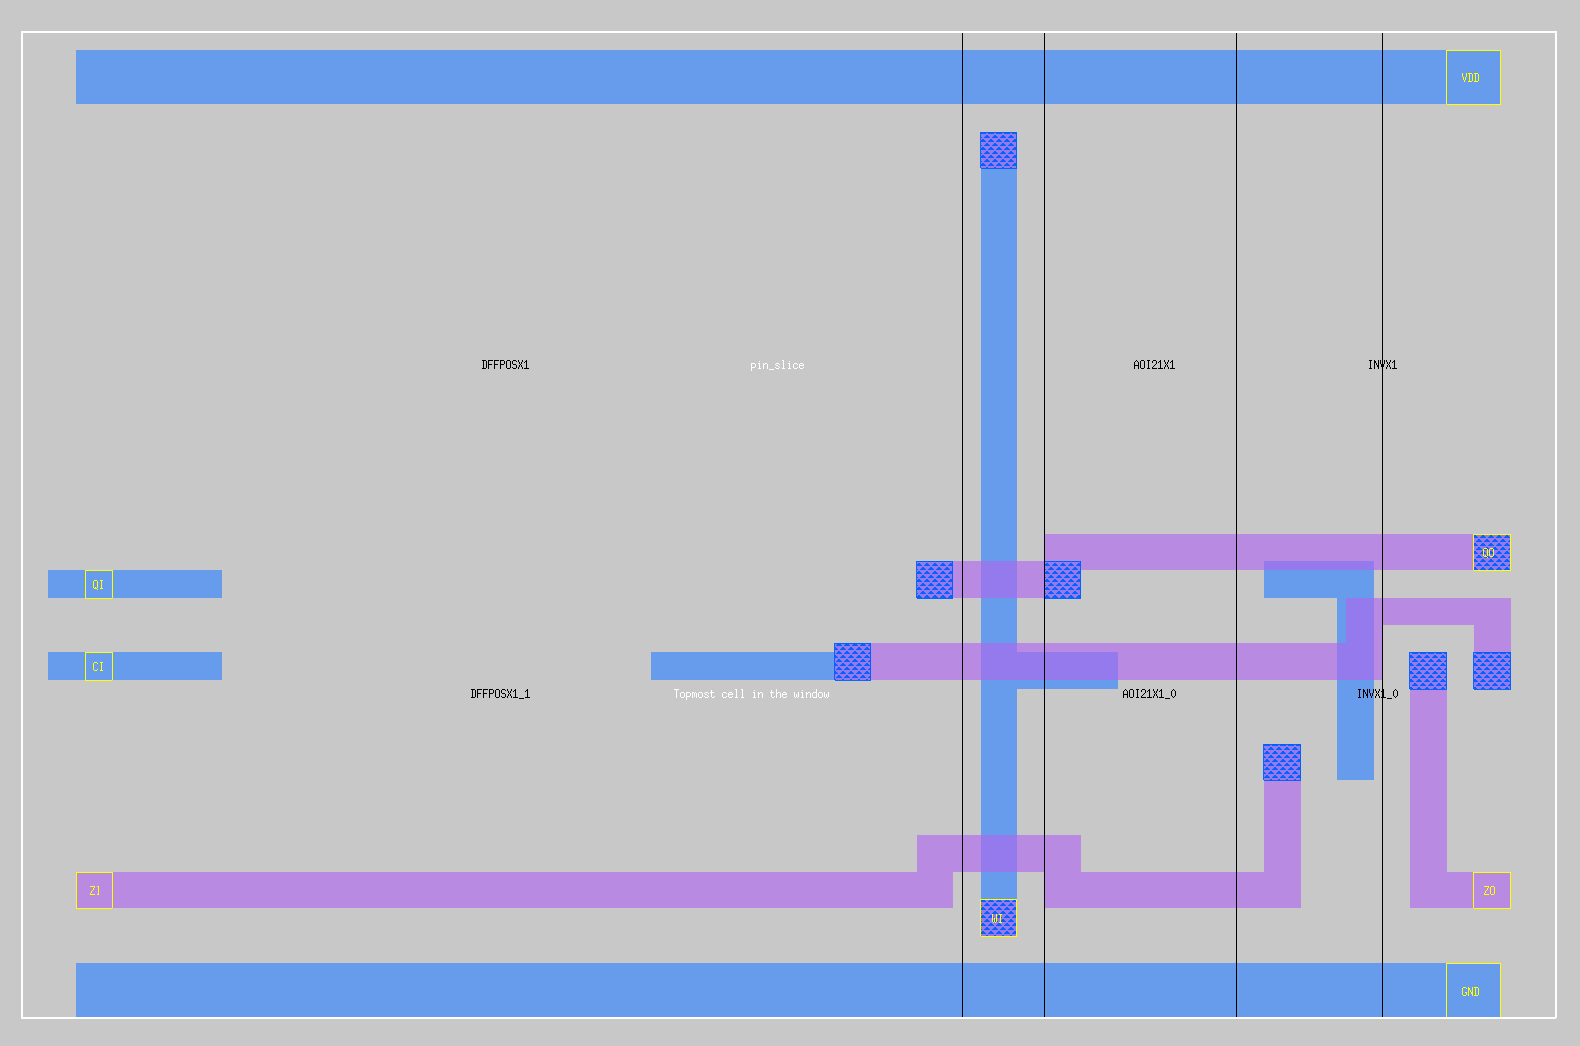
\includegraphics[width=0.75\linewidth]{../../magic/images/pin_slice.png}
            \caption{PIN Slice Layout}
        \end{figure}
        \begin{figure}[H]
            \centering
            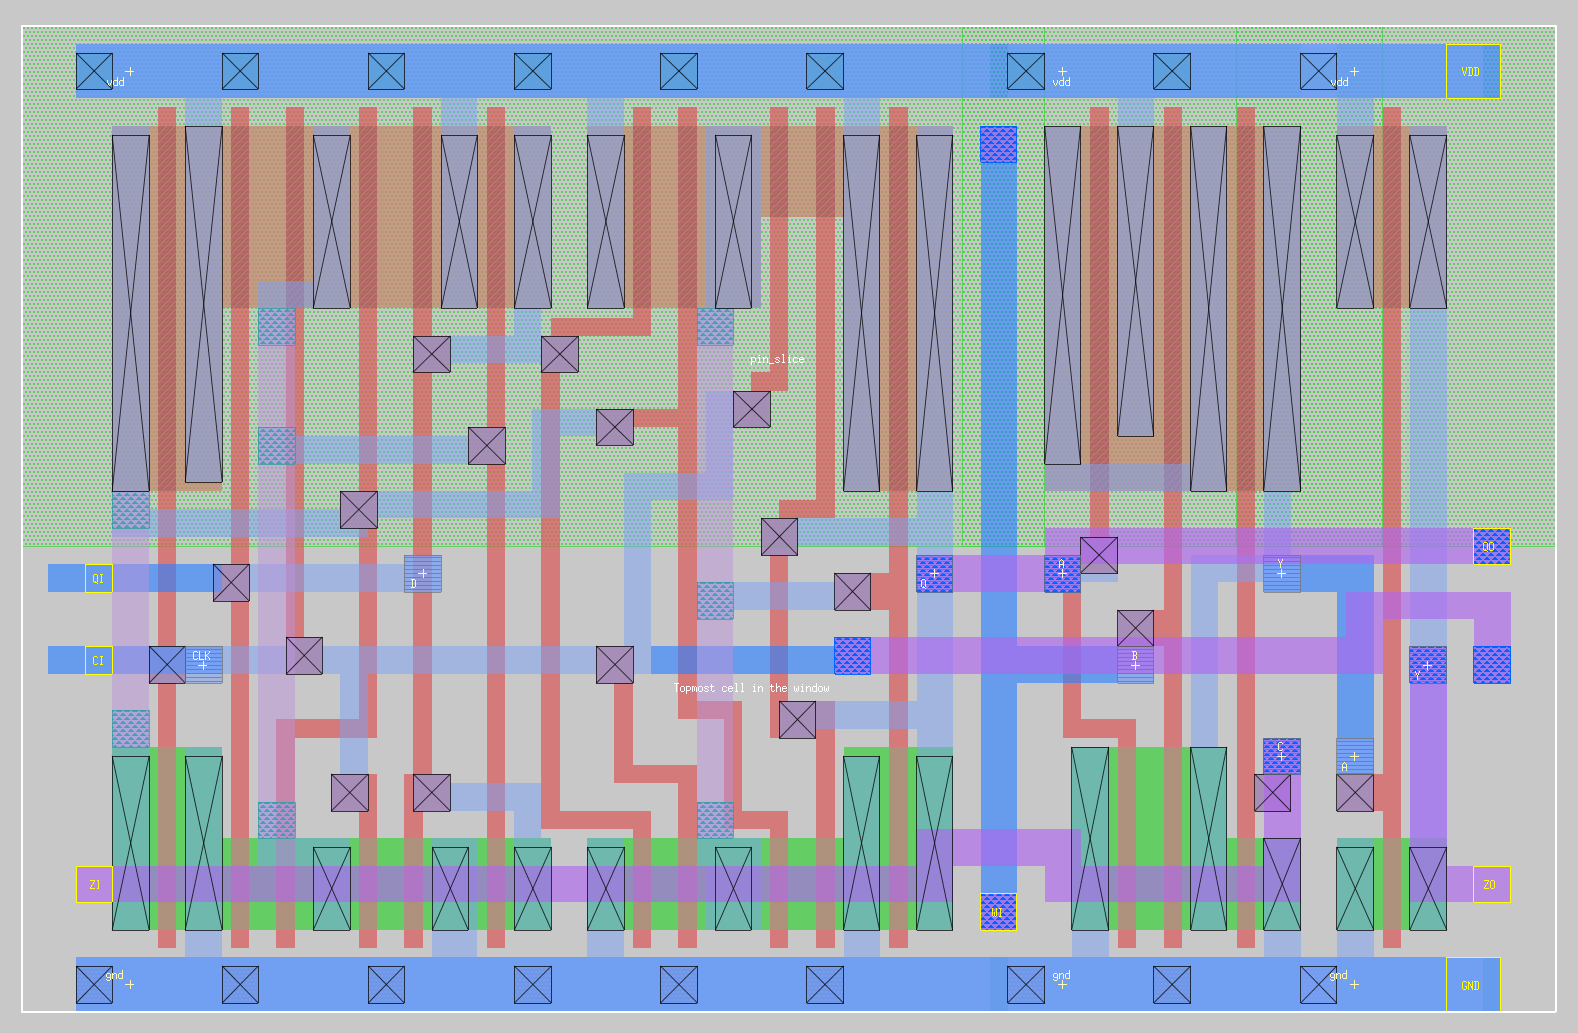
\includegraphics[width=0.75\linewidth]{../../magic/images/pin_slice_internal.png}
            \caption{PIN Slice Layout Internal}
        \end{figure}
    \subsection{Shift Slice Layout}
        Like the PIN slice, the Shift slice layout consists of 3 cells from the provided library.
        Again, we chose to keep a linear layout to maintain a uniform power rail between slices.
        Also, like the PIN slice, the connections in and out of this slice are laid out in such a manner
        that allows for direct patterning of slices with no additional work required.
        \begin{figure}[H]
            \centering
            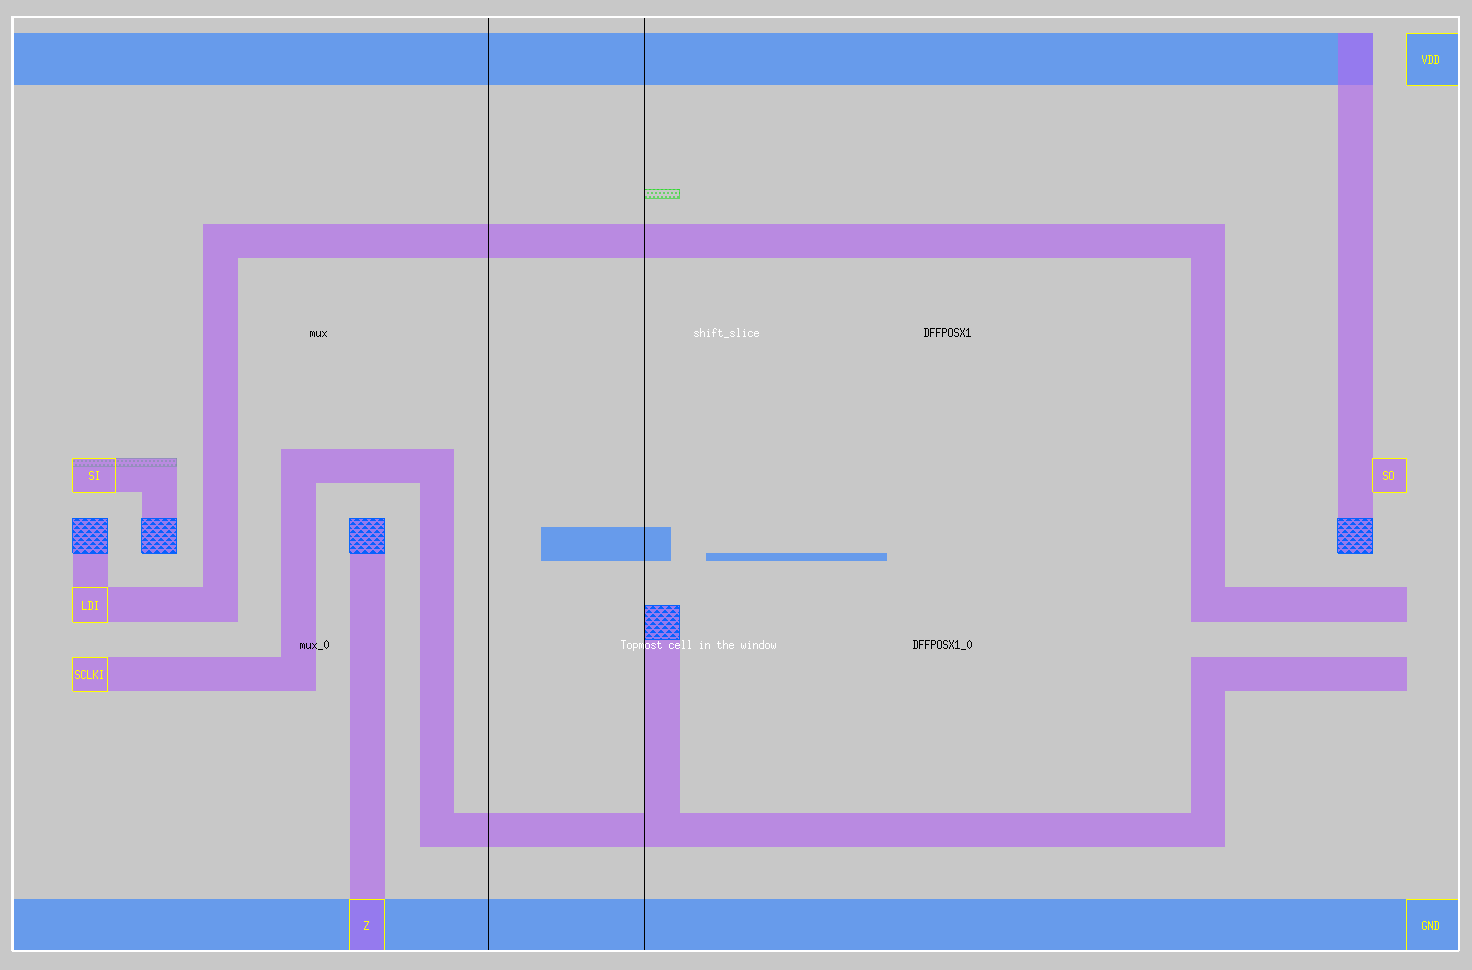
\includegraphics[width=0.75\linewidth]{../../magic/images/shift_slice.png}
            \caption{PIN Slice Layout}
        \end{figure}
        \begin{figure}[H]
            \centering
            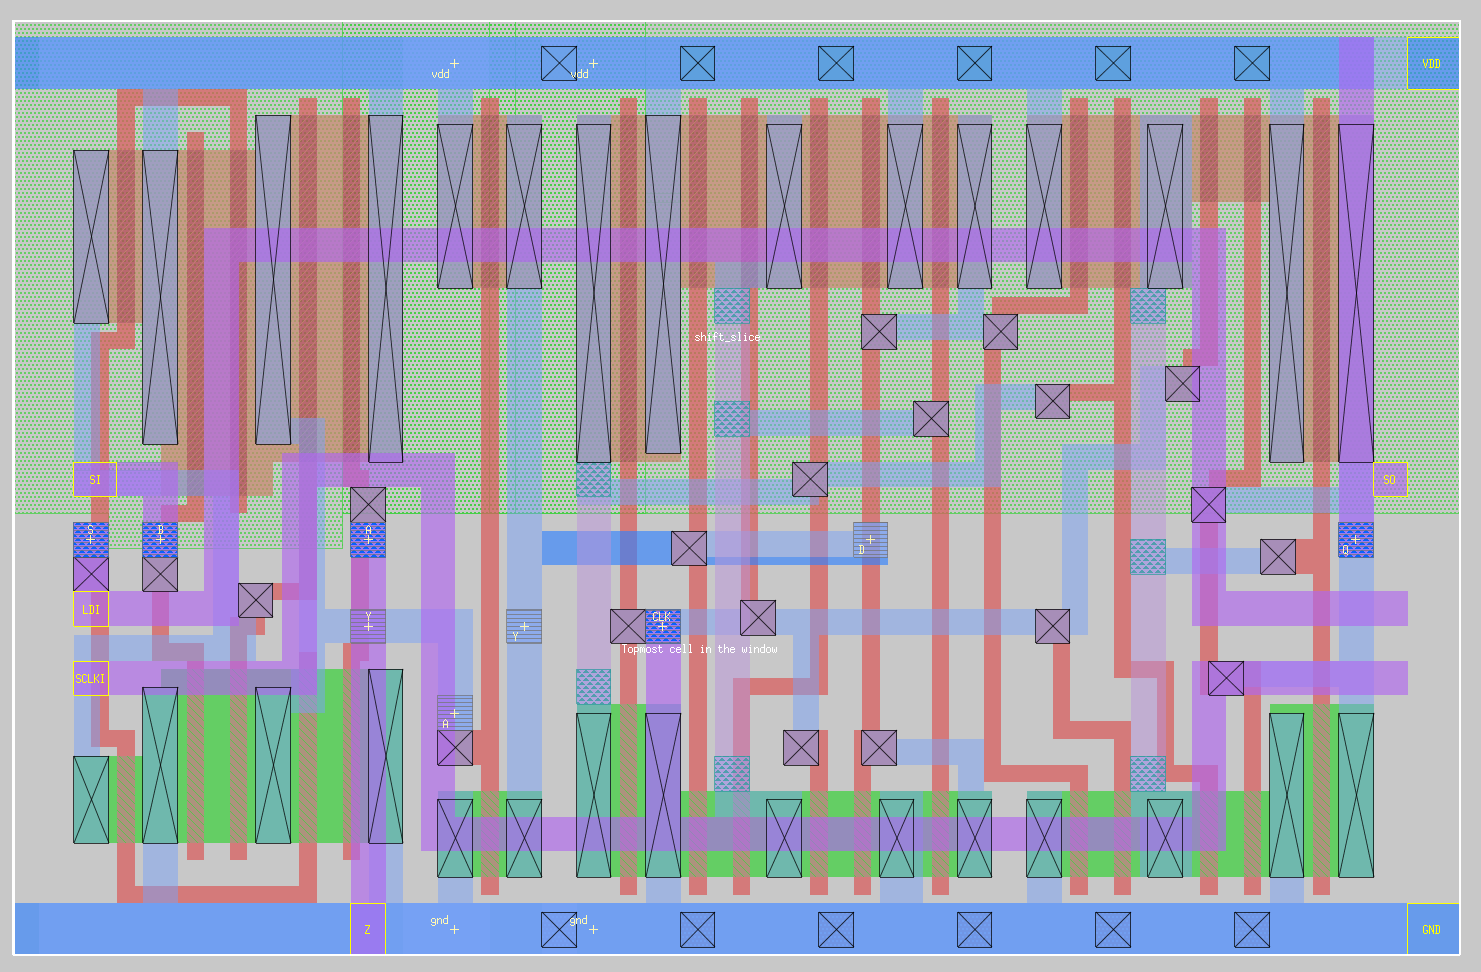
\includegraphics[width=0.75\linewidth]{../../magic/images/shift_slice_internal.png}
            \caption{PIN Slice Layout Internal}
        \end{figure}

\newpage
\section{Slice IRSIM Results}

    \subsection{PIN Slice IRSIM Results}

        In order to test the PIN slice functionally a Python script was
        developed that translates our VHDL testbench patterns into a IRSIM
        command file. The output CMD file is not included here because of its
        length and the fact that it can be inferred from the Python script shown
        below.

        \lstinputlisting[caption=Python PIN Slice IRSIM CMD File Generator, language=Python]{../../irsim/pin_slice.py}

        The resulting IRSIM waveform, shown below, illustrates that we achieve
        correct functional behavior for our slice layout.

        \begin{figure}[H]
            \centering
            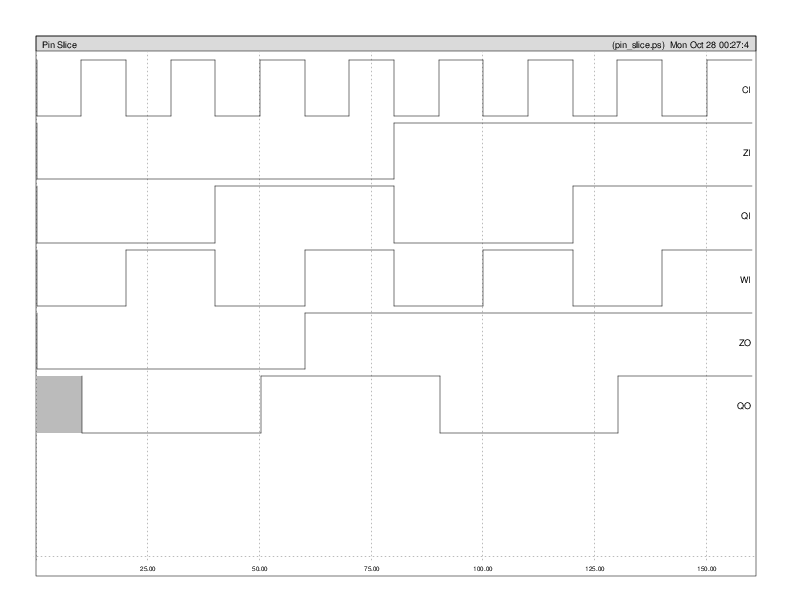
\includegraphics[width=0.75\linewidth]{../../irsim/pin_slice.png}
            \caption{PIN Slice IRSIM Functional Results}
        \end{figure}

        \newpage

        The critical path through the PIN slice is highlighted in red in the
        diagram below. Knowing this path we constructed a simple CMD file to
        toggle the \texttt{qi} pin high and low on two consecutive clock
        cycles. This gives us a rising and falling edge through the critical
        path that we were able to measure using the \texttt{PATH} command in
        IRSIM. 

        \begin{figure}[H]
            \centering
            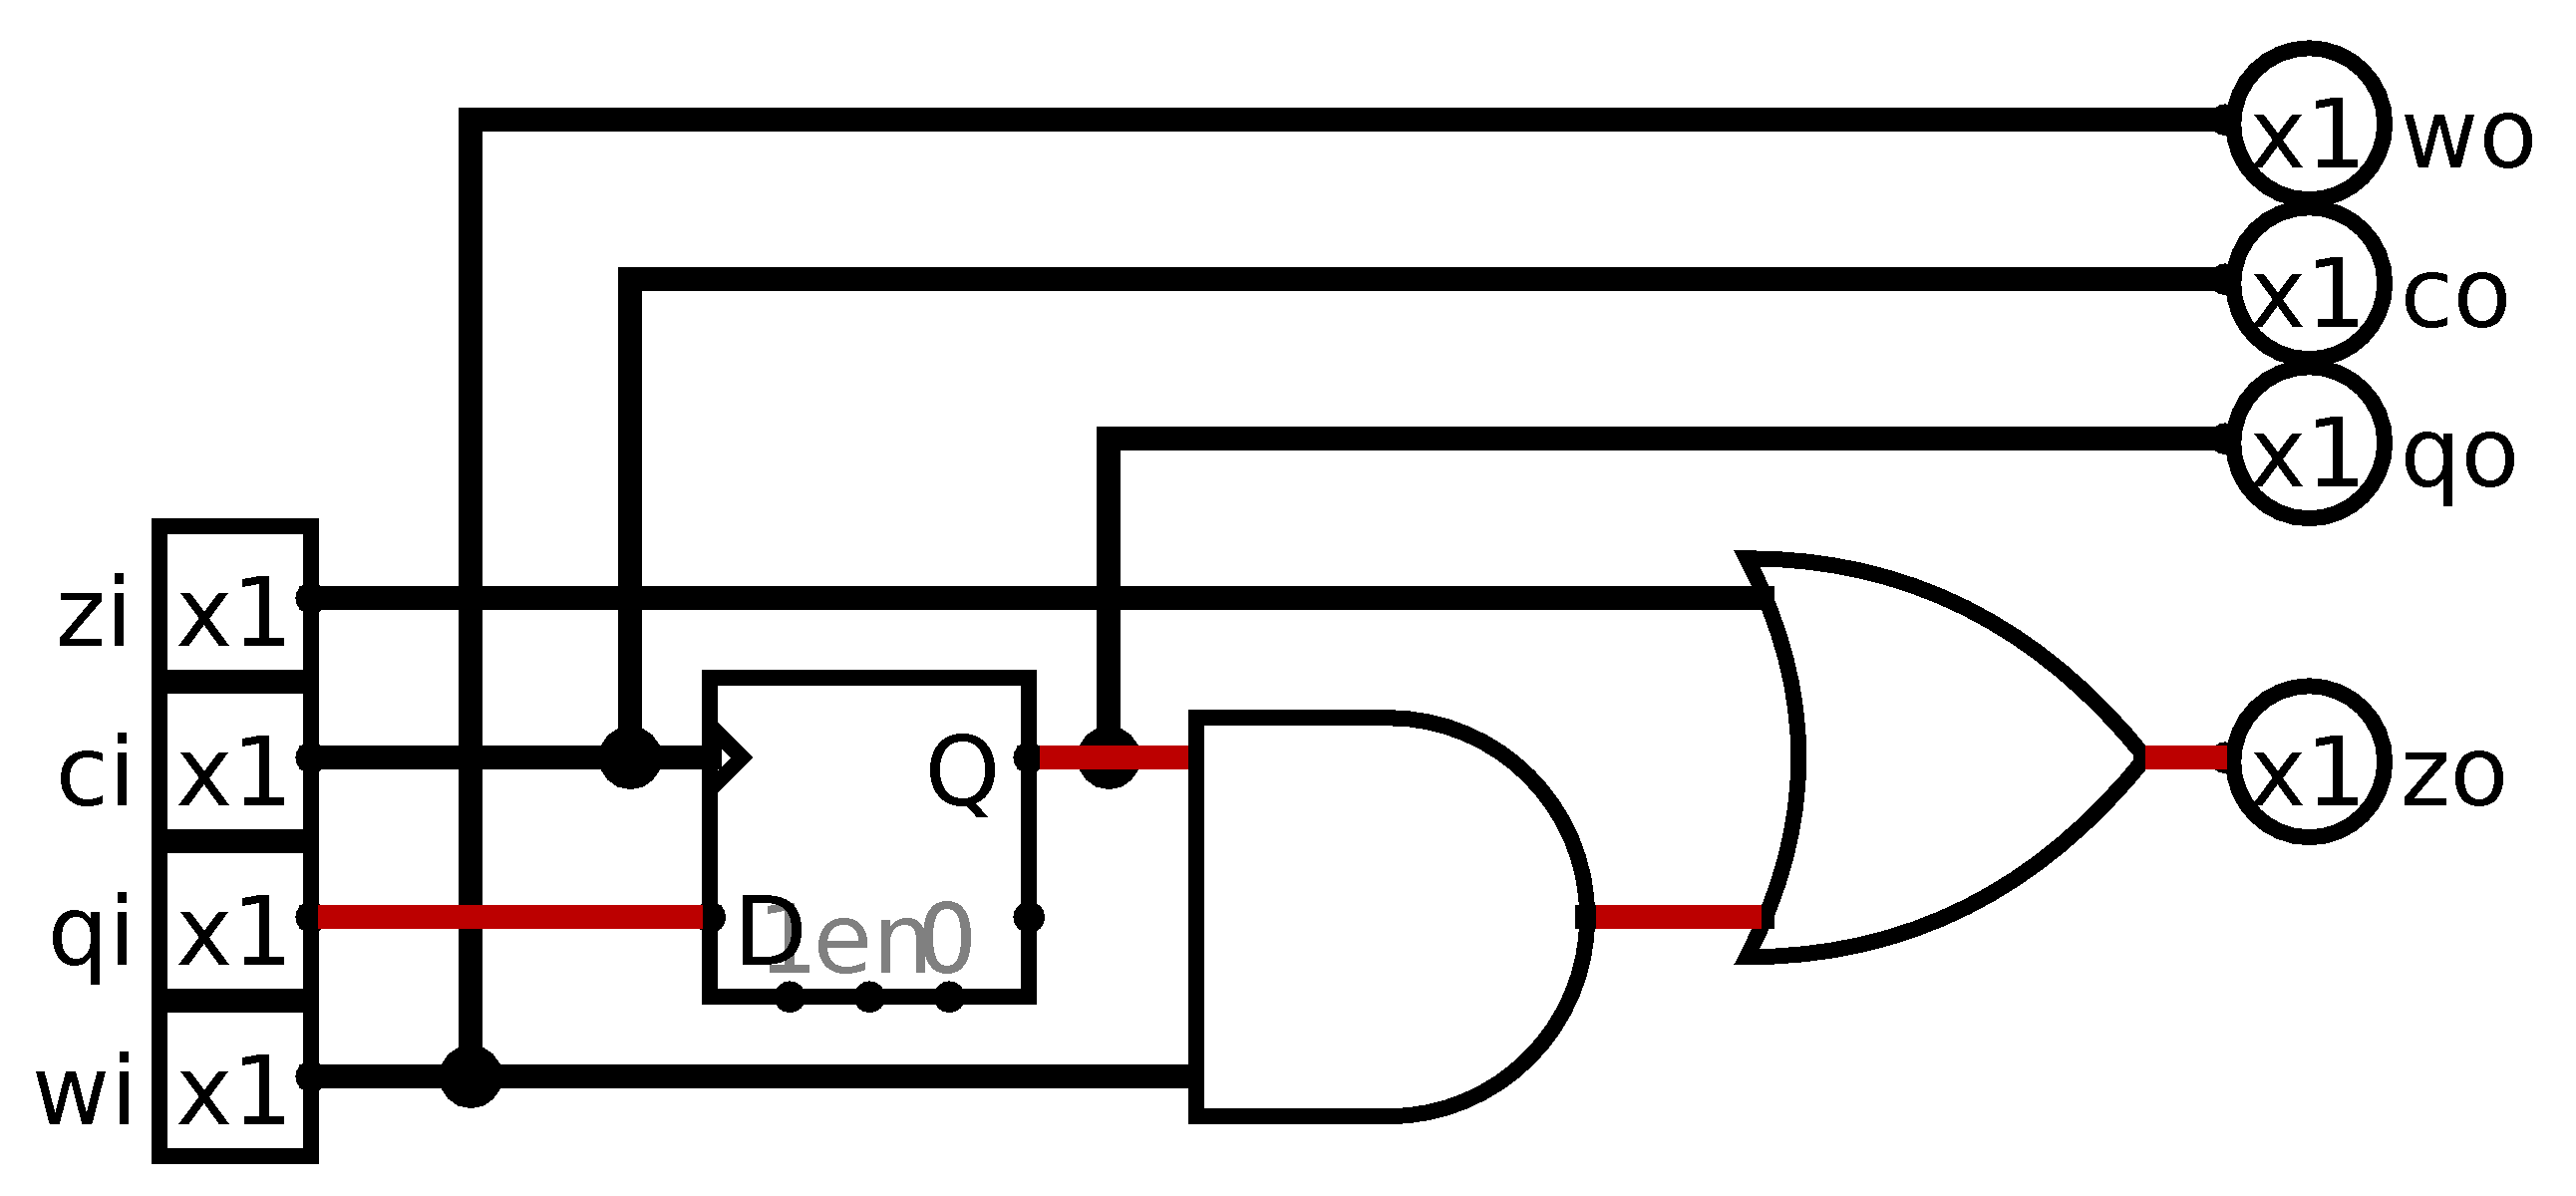
\includegraphics[width=0.75\linewidth]{../../logisim/pin_slice_crit_path.png}
            \caption{PIN Slice Critical Path}
        \end{figure}

        The textual output from IRSIM is shown below:

        \begin{figure}[H]
            \centering
            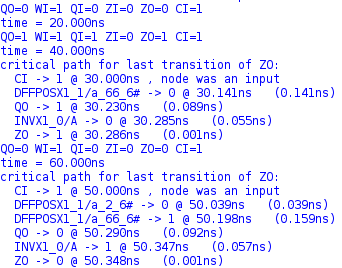
\includegraphics[width=0.5\linewidth]{../../irsim/pin_slice_timing.png}
            \caption{PIN Slice IRSIM Critical Path Delay}
        \end{figure}
        \vspace{\baselineskip}

        Looking at the output we can see the two delays of the critical path.
        The first of the two delays is the output value going from a \texttt{0} to
        a \texttt{1} and the second is the output going from a \texttt{1} to a
        \texttt{0}.  The table below tabulates the two delays and indicates
        that the falling edge delay was the worse of the two.
        \vspace{\baselineskip}

        \begin{table}[H]
            \centering
            \begin{tabular}{crc}
                \toprule
                \textbf{State Change} & \textbf{Delay} & \\
                \midrule
                0 & 0.286n & \\
                1 & 0.348n & WORST \\
                \bottomrule
            \end{tabular}
            \caption{PIN Slice IRSIM Critical Path Delays}
        \end{table}

    \newpage
    \subsection{Shift Slice IRSIM Results}

        Similarly to the PIN slice, for the Shift Slice we used the same Python
        script to generate a CMD file that matched our VHDL testbench patterns.
        The script is shown below:

        \lstinputlisting[caption=Python Shift Slice IRSIM CMD File Generator, language=Python]{../../irsim/shift_slice.py}

        Looking at the results we can see that our Shift Slice performs as
        expected and matches our VHDL simulations.

        \begin{figure}[H]
            \centering
            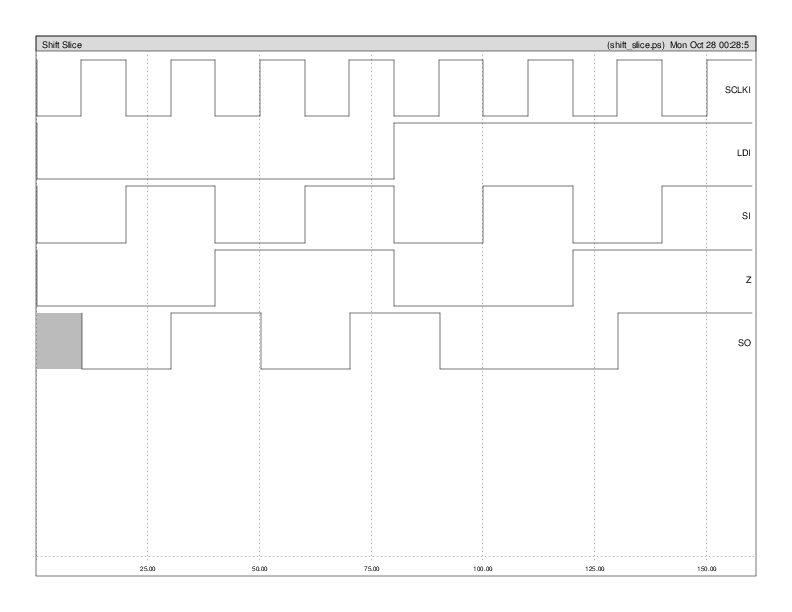
\includegraphics[width=0.75\linewidth]{../../irsim/shift_slice.png}
            \caption{Shift Slice IRSIM Functional Results}
        \end{figure}

        \newpage

        The critical path through the shift slice is highlighted in red in the
        diagram below. Again, knowing this path we constructed a simple CMD
        file to drive a pulse through the path.

        \begin{figure}[H]
            \centering
            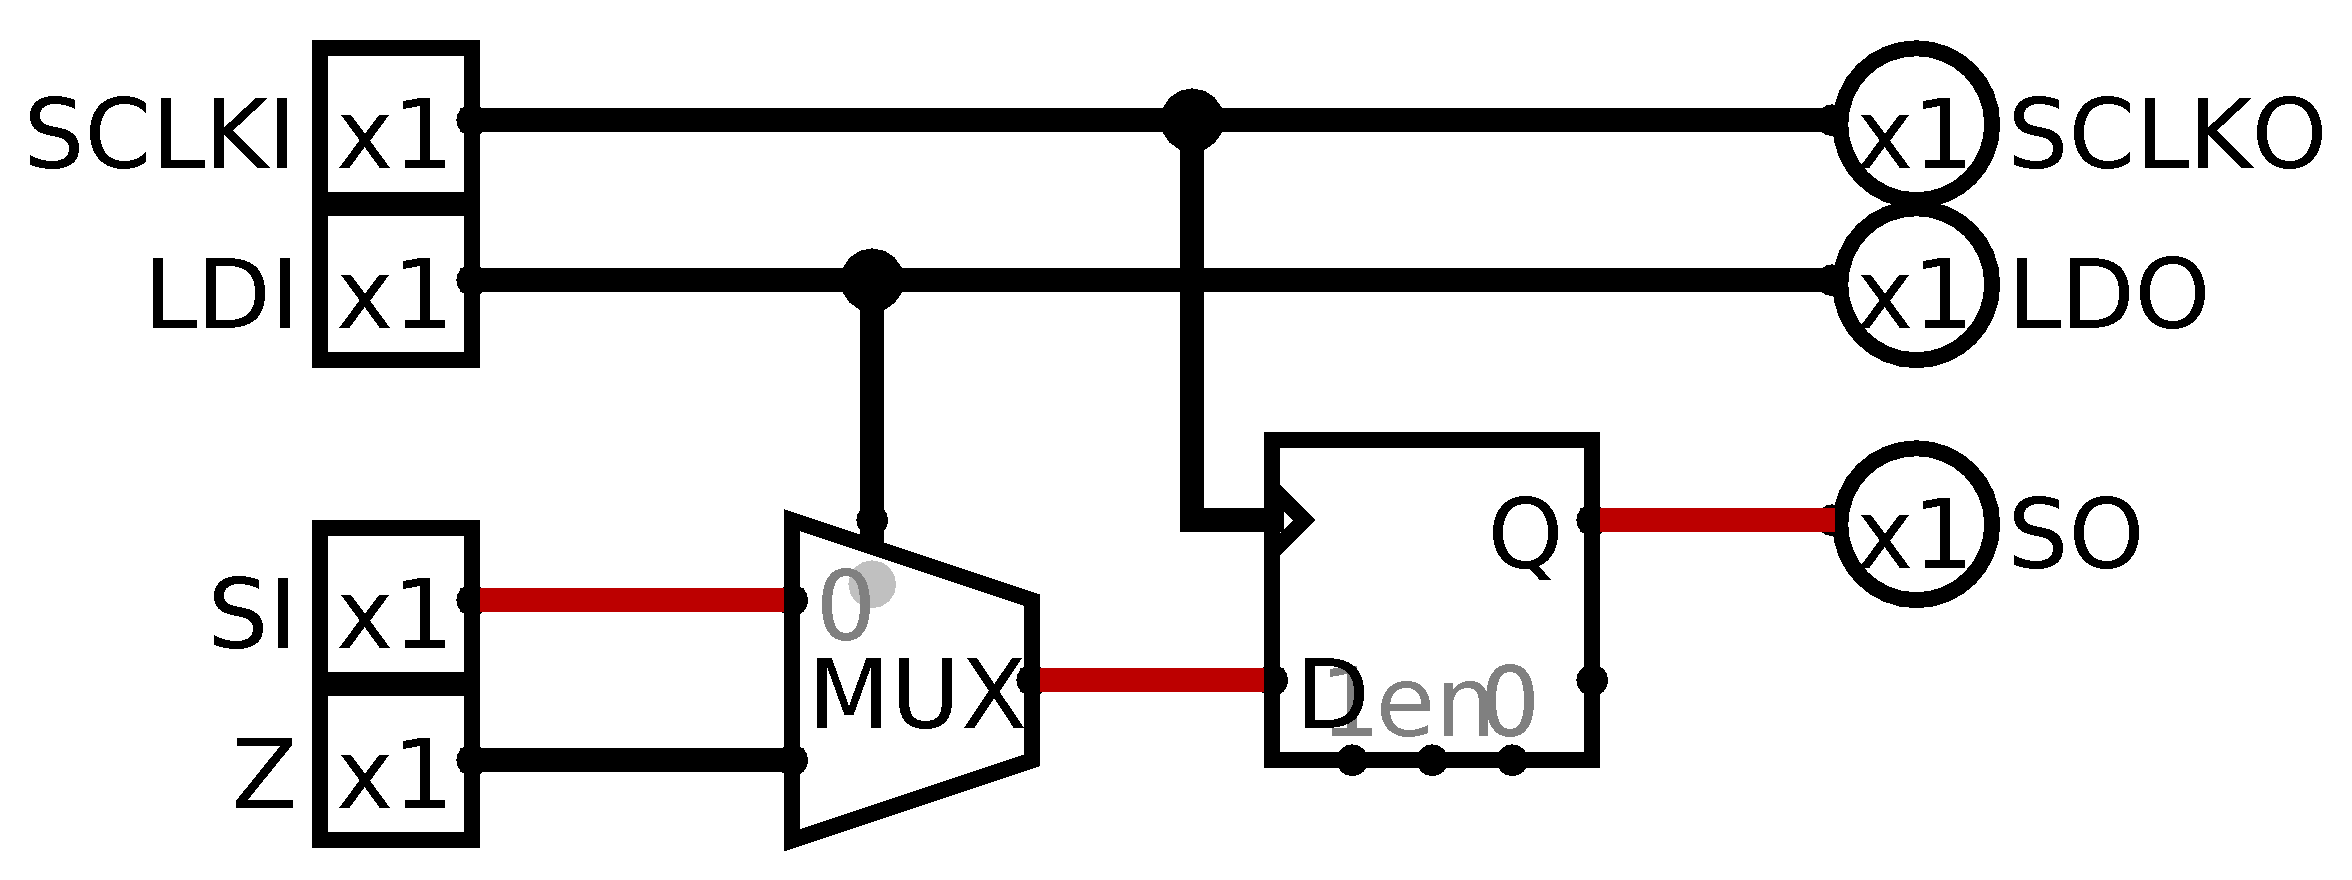
\includegraphics[width=\linewidth]{../../logisim/shift_slice_crit_path.png}
            \caption{Shift Slice Critical Path}
        \end{figure}

        The textual output from IRSIM, shown below, provides us with two
        critical path delays one for the rising edge of the output and one for
        the falling edge.

        \begin{figure}[H]
            \centering
            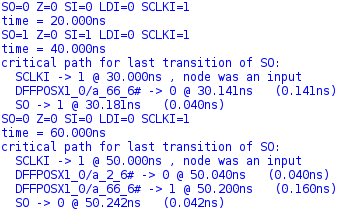
\includegraphics[]{../../irsim/shift_slice_timing.png}
            \caption{Shift Slice IRSIM Critical Path Delay}
        \end{figure}
        \vspace{\baselineskip}

        Looking at the output we can see that again the falling edge has a
        greater propagation delay through the path. The table below summarizes
        the results for this slice.
        \vspace{\baselineskip}

        \begin{table}[H]
            \centering
            \begin{tabular}{crc}
                \toprule
                \textbf{State Change} & \textbf{Delay} & \\
                \midrule
                0 & 0.181n & \\
                1 & 0.242n & WORST \\
                \bottomrule
            \end{tabular}
            \caption{Shift Slice IRSIM Critical Path Delays}
        \end{table}


\newpage
\section{Slice Spice Results}

    \subsection{PIN Slice Spice Results}

        We wanted to be able to functionally test our slices in HSpice in
        addition to analyzing the propagation delay. To do this another Python
        script was written that took our test patterns and wrote out the
        required Piecewise Linear (PWL) statements to generate them.

        \lstinputlisting[caption=Python PIN Slice Spice File Generator, language=Python]{../../spice/pin_slice.py}

        In the figure below we can see the result of our functional Spice test.
        As you can see, it again matches our expected functionality once again
        proving the slice is operating correctly.

        \begin{figure}[H]
            \centering
            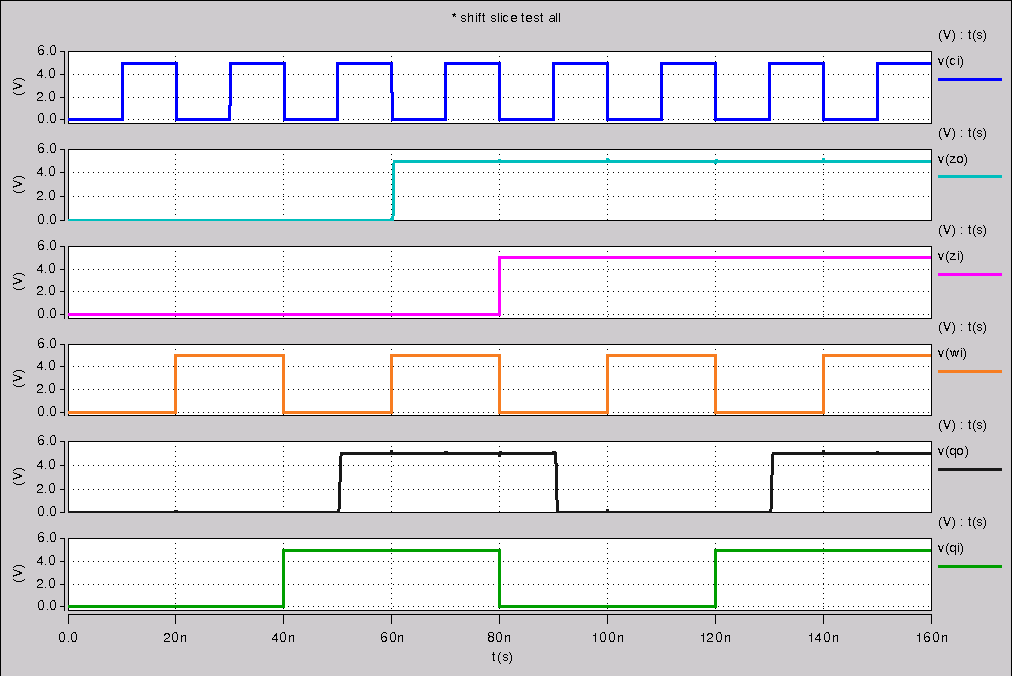
\includegraphics[width=0.65\linewidth]{../../spice/pin_slice_all.png}
            \caption{PIN Slice Spice Functional Results}
        \end{figure}

        \newpage

        In order to measure the critical path delay the patterns in the above
        Python program were modified to simply toggle the input line
        \texttt{QI}. The resulting output was then measured against the input
        clock \texttt{CI} to obtain the delays for both rising and falling
        edges.

        \begin{figure}[H]
            \centering
            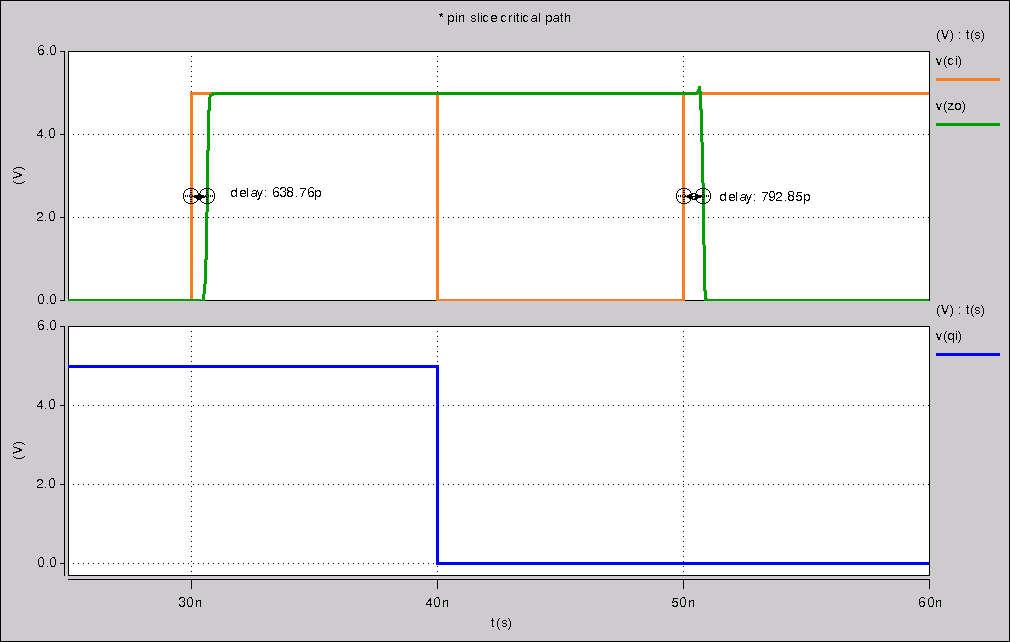
\includegraphics[width=0.75\linewidth]{../../spice/pin_slice_crit_path.png}
            \caption{PIN Slice Spice Critical Path Delay}
        \end{figure}

        \vspace{\baselineskip}
        The delay times for each of these state changes is tabulated below.

        \begin{table}[H]
            \centering
            \begin{tabular}{crc}
                \toprule
                \textbf{State Change} & \textbf{Delay} & \\
                \midrule
                0 & 0.638n & \\
                1 & 0.792n & WORST \\
                \bottomrule
            \end{tabular}
            \caption{PIN Slice Spice Critical Path Delays}
        \end{table}

    \newpage

    \subsection{Shift Slice Spice Results}

        Similarly to the PIN slice spice tests we again wanted to be able to
        test the logical functionality of our slice in HSpice. The same Python
        script was utilized with a few tweaks to the variable names and pattern
        definitions in order to match this slice.

        \lstinputlisting[caption=Python Shift Slice Spice File Generator, language=Python]{../../spice/shift_slice.py}

        From the output waveform below we can see that our slice performed as
        we expected at a logical level.

        \begin{figure}[H]
            \centering
            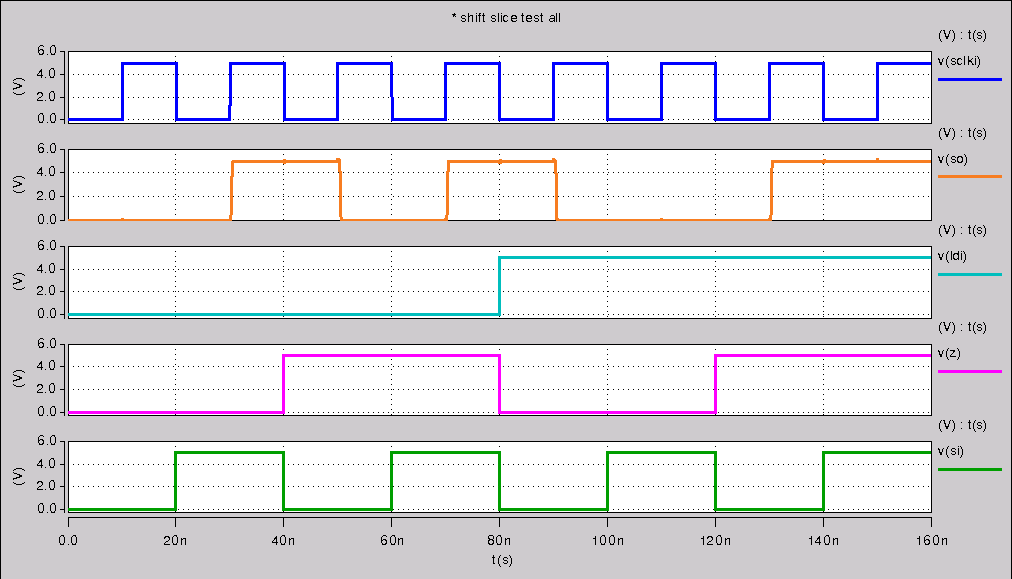
\includegraphics[width=0.75\linewidth]{../../spice/shift_slice_all.png}
            \caption{Shift Slice Spice Functional Results}
        \end{figure}

        \newpage

        To obtain the delays the input pattern was modified to send a single
        pulse through the critical path.  The output was then referenced to the
        input clock in order to measure the propagation delay of each edge.

        \begin{figure}[H]
            \centering
            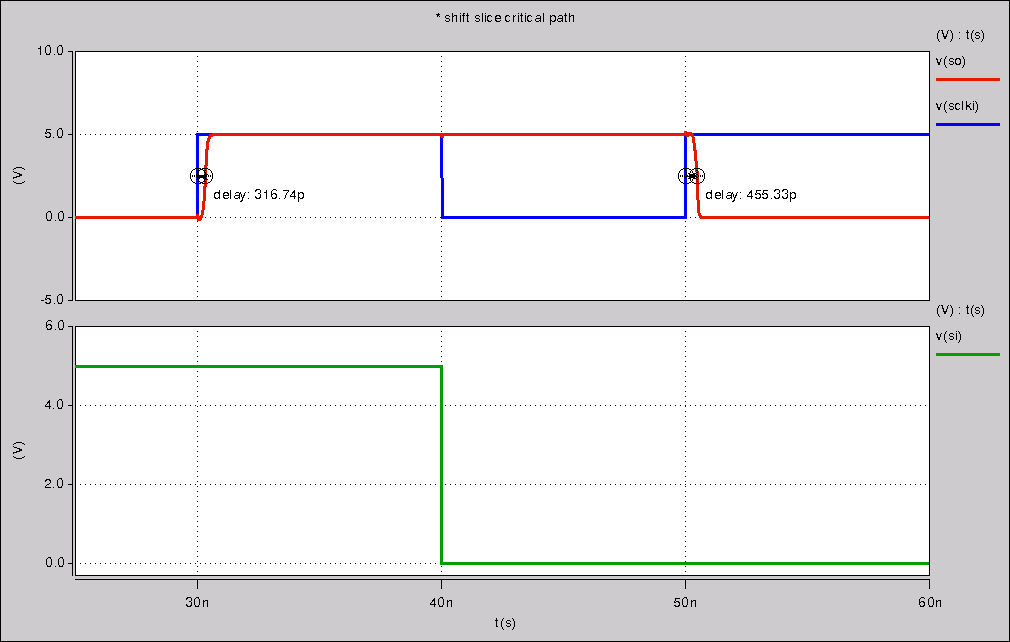
\includegraphics[width=0.75\linewidth]{../../spice/shift_slice_crit_path.png}
            \caption{Shift Slice Spice Critical Path Delay}
        \end{figure}

        \vspace{\baselineskip}

        The delays of the rising and falling edges are tabulated below.

        \begin{table}[H]
            \centering
            \begin{tabular}{crc}
                \toprule
                \textbf{State Change} & \textbf{Delay} & \\
                \midrule
                0 & 0.316n & \\
                1 & 0.455n & WORST \\
                \bottomrule
            \end{tabular}
            \caption{Shift Slice Spice Critical Path Delays}
        \end{table}


    \newpage
\section{Gate Spice Results}
    In order to figure out the worst case delay of each gate we generate an
    exhaustive list of input patterns that toggle the gate inputs in every such
    state that results in the outputs changing. With this we are trying to find
    the input state change that causes the worst case delay. We then measure
    each delay using the \texttt{.measure} directive and look for worst
    delay time.

    \subsection{DFFPOSX1 Spice Results}

        \lstinputlisting[caption=Python DFFPOSX1 Spice File Generator, language=Python]{../../spice/dffposx1.py}

        \begin{figure}[H]
            \centering
            \begin{minipage}[t]{.50\textwidth}
                \vspace{0pt}
                \centering
                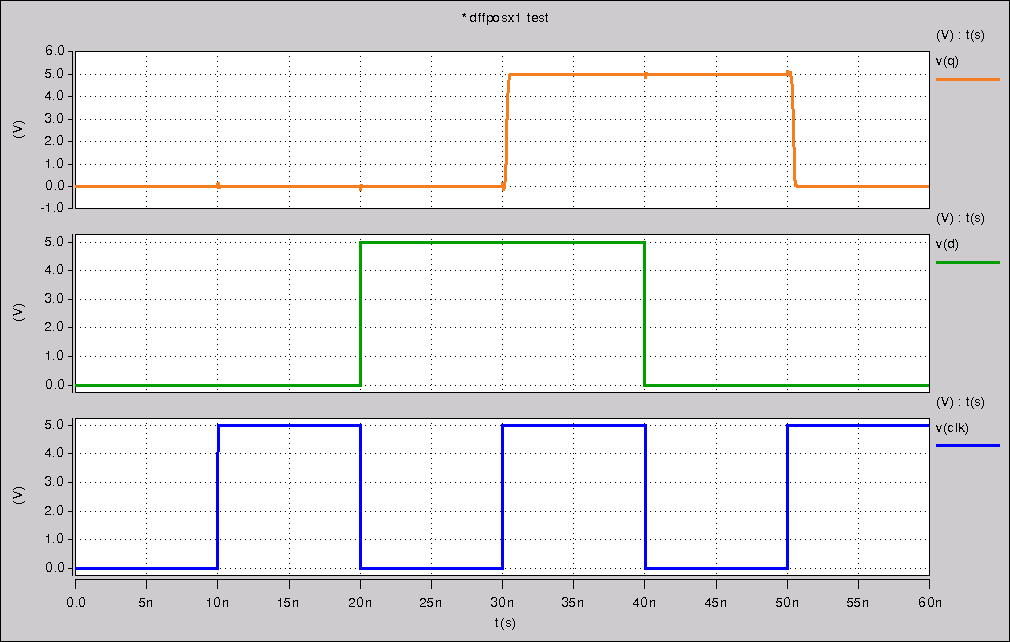
\includegraphics[width=\linewidth]{../../spice/dffposx1.png}
                \caption{DFFPOSX1 Spice Results}
            \end{minipage}
            \hfill
            \begin{minipage}[t]{.45\textwidth}
                \vspace{0pt}

                \begin{table}[H]
                    \centering
                    \begin{tabular}{crc}
                        \toprule
                        \textbf{State Change} & \textbf{Delay} & \\
                        \midrule
                        0 & 0.3011n & \\
                        1 & 0.4257n & WORST \\
                        \bottomrule
                    \end{tabular}
                    \caption{DFFPOSX1 Delays}
                \end{table}
            \end{minipage}
        \end{figure}

    \newpage
    \subsection{AOI21X1 Spice Results}

        \lstinputlisting[caption=Python AOI21X1 Spice File Generator, language=Python]{../../spice/aoi21x1.py}

        \begin{figure}[H]
            \centering
            \begin{minipage}[t]{.50\textwidth}
                \vspace{0pt}
                \centering
                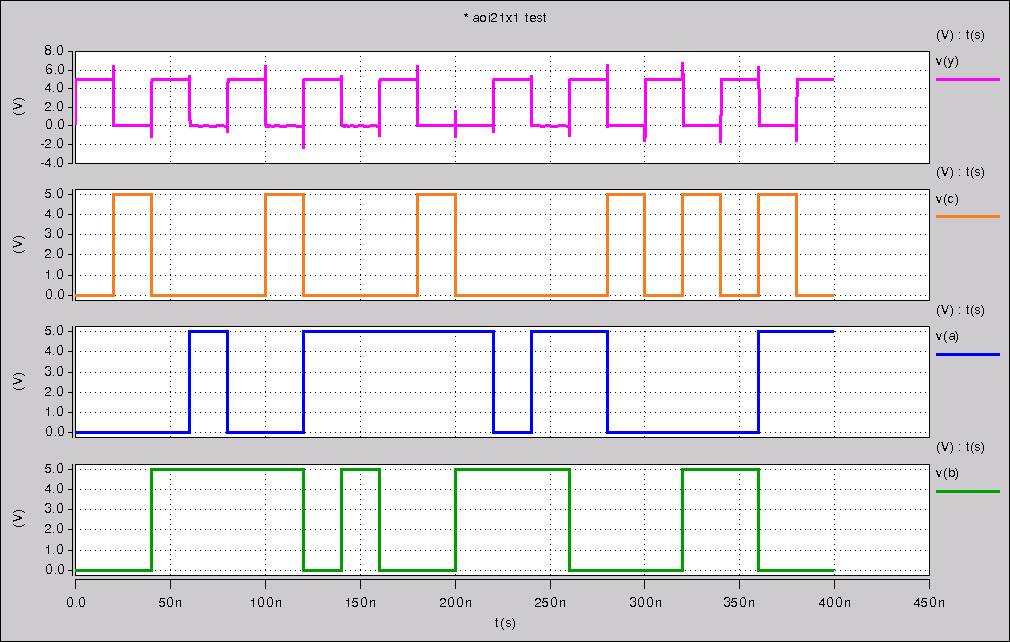
\includegraphics[width=\linewidth]{../../spice/aoi21x1.png}
                \caption{AOI21X1 Spice Results}
            \end{minipage}
            \hfill
            \begin{minipage}[t]{.45\textwidth}
                \vspace{0pt}
                \begin{table}[H]
                    \centering
                    \begin{tabular}{crc}
                        \toprule
                        \textbf{State Change} & \textbf{Delay} & \\
                        \midrule
                        0 & 0.1075n & \\
                        1 & 0.1577n & WORST \\
                        2 & 0.1207n & \\
                        3 & 0.1434n & \\
                        4 & 0.1076n & \\
                        5 & 0.1457n & \\
                        6 & 0.1150n & \\
                        7 & 0.0491n & \\
                        8 & 0.0871n & \\
                        9 & 0.0580n & \\
                        \bottomrule
                    \end{tabular}
                    \caption{AOI21X1 Delays}
                \end{table}
            \end{minipage}
        \end{figure}

        \newpage
        \subsection{MUX2X1 Spice Results}
        \lstinputlisting[caption=Python MUX2X1 Spice File Generator, language=Python]{../../spice/mux2x1.py}
        \begin{figure}[H]
            \centering
            \begin{minipage}[t]{.50\textwidth}
                \vspace{0pt}
                \centering
                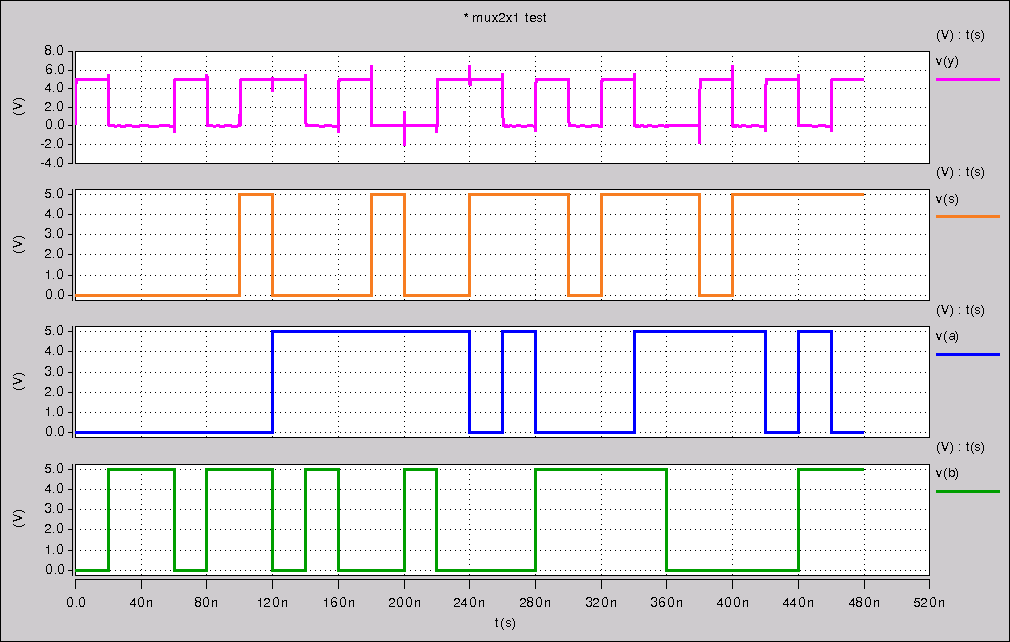
\includegraphics[width=\linewidth]{../../spice/mux2x1.png}
                \caption{MUX2X1 Spice Results}
            \end{minipage}
            \hfill
            \begin{minipage}[t]{.45\textwidth}
                \vspace{0pt}
                \begin{table}[H]
                    \centering
                    \begin{tabular}{crc}
                        \toprule
                        \textbf{State Change} & \textbf{Delay} & \\
                        \midrule
                        0  & 0.1536n & \\
                        1  & 0.1342n & \\
                        2  & 0.2569n & \\
                        3  & 0.1542n & \\
                        4  & 0.0832n & \\
                        5  & 0.1340n & \\
                        6  & 0.1390n & \\
                        7  & 0.2571n & WORST \\
                        8  & 0.1391n & \\
                        9  & 0.0788n & \\
                        10 & 0.1464n & \\
                        11 & 0.1467n & \\
                        \bottomrule
                    \end{tabular}
                    \caption{MUX2X1 Delays}
                \end{table}
            \end{minipage}
        \end{figure}


        \newpage
        \subsection{INVX1 Spice Results}
        \lstinputlisting[caption=Python INVX1 Spice File Generator, language=Python]{../../spice/invx1.py}
        \begin{figure}[H]
            \centering
            \begin{minipage}[t]{.50\textwidth}
                \vspace{0pt}
                \centering
                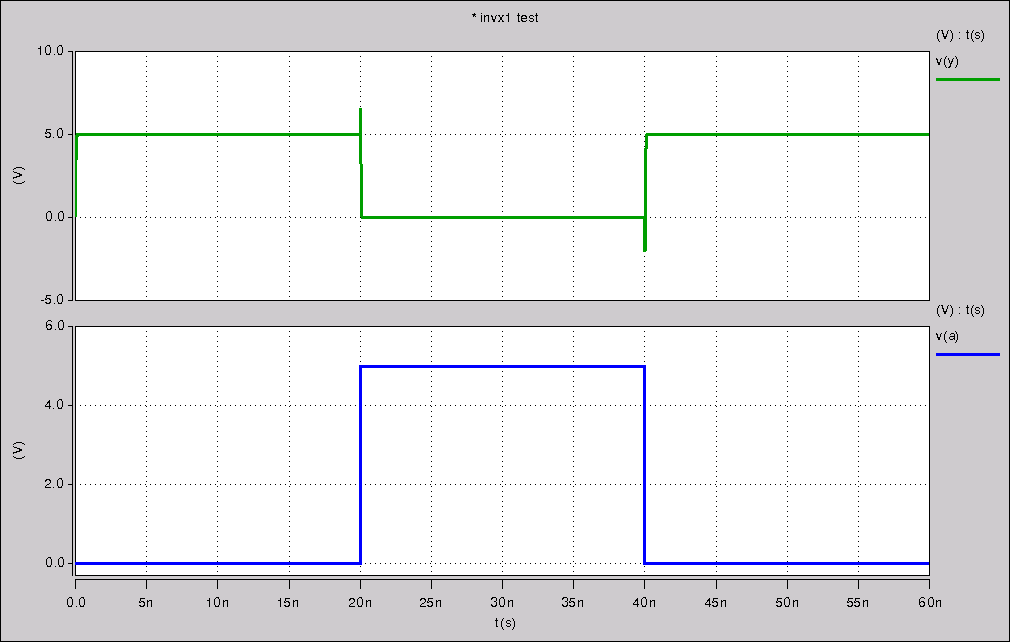
\includegraphics[width=\linewidth]{../../spice/invx1.png}
                \caption{INVX1 Spice Results}
            \end{minipage}
            \hfill
            \begin{minipage}[t]{.45\textwidth}
                \vspace{0pt}
                \begin{table}[H]
                    \centering
                    \begin{tabular}{crc}
                        \toprule
                        \textbf{State Change} & \textbf{Delay} & \\
                        \midrule
                        0 & 0.0550n & WORST \\
                        1 & 0.0407n & \\
                        \bottomrule
                    \end{tabular}
                    \caption{INVX1 Delays}
                \end{table}
            \end{minipage}
        \end{figure}

    \vspace{2\baselineskip}
    \subsection{Leaf Component Delay Summary}

        A table summarizing the worst delays for each gate is shown below.

        \begin{table}[H]
            \centering
            \begin{tabular}{lc}
                \toprule
                \textbf{Component} & \textbf{Worst Delay} \\
                \midrule
                AOI21X1  & 0.1577n \\
                DFFPOSX1 & 0.4257n \\
                INVX1    & 0.0550n \\
                MUX2X1   & 0.2571n \\
                \bottomrule
            \end{tabular}
            \caption{Worst Case Delay Summary}
        \end{table}

\newpage
\section{VHDL Models With Timing}
    Using the worst case leaf delays, found above, we updated our VHDL models
    in order to take the delay into account.  All other modules and testbenches
    required no changes and were left as is.
    \lstinputlisting[caption=AOI21X1 VHDL Module With Delay]{../../vhdl/aoi21x1.vhd}
    \lstinputlisting[caption=DFFPOSX1 VHDL Module With Delay]{../../vhdl/dffposx1.vhd}
    \lstinputlisting[caption=INVX1 VHDL Module With Delay]{../../vhdl/invx1.vhd}
    \lstinputlisting[caption=MUX2X1 VHDL Module With Delay]{../../vhdl/mux2x1.vhd}
\section{VHDL Testbench Results With Timing}

    \subsection{VHDL Slice Testbench With Delays Waveform}

        Looking at the outputs of the slice test benches we can see that they
        perform as expected and match not only the original test benches but
        the IRSIM and HSpice functional test waveforms.  Since we know the
        delays of each gate and which gates are in each cell there is no need
        to show a zoomed in waveform illustrating the delay in VHDL, we can
        simply add up the delays manually as there is no other delay introduced
        in the simulation.

        \begin{figure}[H]
            \centering
            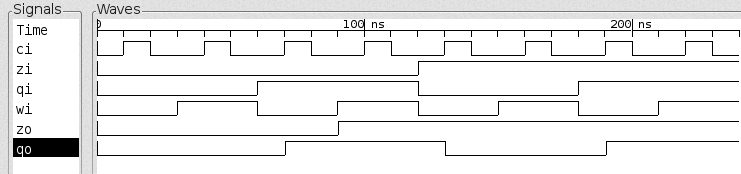
\includegraphics[width=0.8\linewidth]{../../doc/vhdl_sim_pics/pin_slice_with_delays.png}
            \caption{VHDL PIN Slice With Delays Waveform}
        \end{figure}

        \begin{figure}[H]
            \centering
            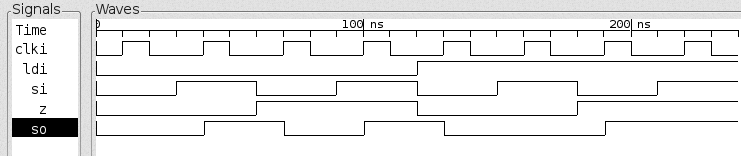
\includegraphics[width=0.8\linewidth]{../../doc/vhdl_sim_pics/shift_slice_with_delays.png}
            \caption{VHDL Shift Slice With Delays Waveform}
        \end{figure}

    \subsection{VHDL Top Level Testbench With Delays Waveform}

        Looking at the results of the top level testbenches for both normal and
        test mode we can see that they are again identical to the waveforms
        captured without delays.  Additionally, since our testbench is
        exhaustive and self-checking we can be certain that the delays did not
        introduce any corner cases that one might miss if they are spot checking
        manually.
        \begin{figure}[H]
            \centering
            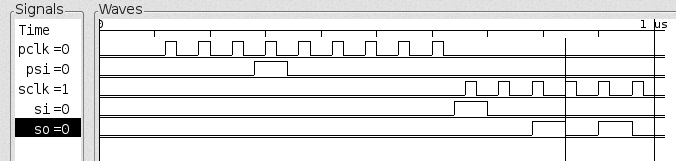
\includegraphics[width=0.8\linewidth]{../../doc/vhdl_sim_pics/top.png}
            \caption{VHDL Top Level Functional Test Bench With Delays Waveform}
        \end{figure}

        \begin{figure}[H]
            \centering
            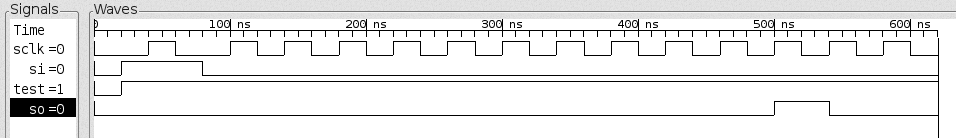
\includegraphics[width=0.8\linewidth]{../../doc/vhdl_sim_pics/top_test.png}
            \caption{VHDL Top Level Test Mode Test Bench With Delays Waveform}
        \end{figure}

\newpage
\section{Final Simulation Comparision}

    Taking a look at the final critical path delay summary we can see that
    there is a bit of discrepancy between the different simulations. We are not
    one hundred percent certain why this exists but our best guesses lead to
    explaining it as an artifact of the different simulation techniques used by
    each simulator and what parameters they take into account. While there are
    slight discrepancies all the worst case delays are under 1ns which gives us
    a theoretical \textbf{max clock speed of 1.3GHz}. Since our design is
    basically all shift registers we should also be able to achieve a
    throughput equal to the max clock rate. Once we simulate the full layout,
    which will introduce some long traces between slice rows, we will be able
    to determine a more accurate maximum clock and throughput rates.

    \vspace{\baselineskip}

    \begin{table}[H]
        \centering
        \begin{tabular}{ccc}
            \toprule
            \textbf{Simulation} & \textbf{PIN} & \textbf{Shift} \\
            \midrule
            IRSIM & 0.348n & 0.242n \\
            SPICE & 0.792n & 0.455n \\
            VHDL  & 0.638n & 0.682n \\
            \bottomrule
        \end{tabular}
        \caption{Critical Path Delay Comparison}
    \end{table}

\newpage
\section{Floor Plan}

    The current floorplan that we plan on pursuing is shown below. From initial
    placement testing we believe we will be able to achieve a \textbf{15x15}
    grid of slices. The majority of the core functionality is contained in a
    nice, symmetrically sliced, square. The only additional components that
    fall outside of this model are the 3 MUXs that are required for test mode.
    The floor plan shown below indicates the planned location of all test
    slices and the major components of our design, namely the Shifter and the
    PIN.
    \vspace{\baselineskip}

    \begin{figure}[H]
        \centering
        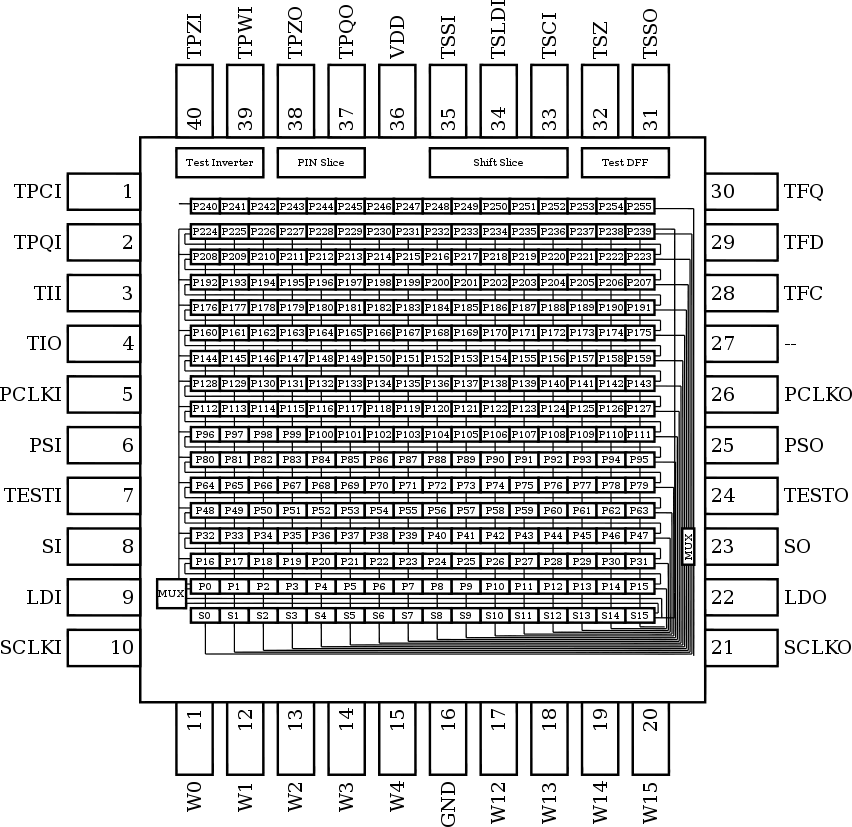
\includegraphics[width=\linewidth]{../floorplan/floorplan.png}
        \caption{Floor Plan Diagram}
        \label{fig:floorplan}
    \end{figure}

\section{Major Design Decisions}

The major design decisions revolved mainly around the layout of each slice. We
knew we wanted to come up with a design that would allow us to tile with
minimal effort.  Achieving this goal was not necessarily difficult but it
required an iterative design process to break out each signal in such as way
that would allow them to directly connect together.

Another decision that was made early on was simply `which cells should we use?'.
While some parts of our slice, such as the D Flip Flop, were obvious choices
others were more flexible. In the schematic representation of our PIN slice we
show a 2 input AND gate feeding into a 2 input OR gate. As it turns out, the
provided library has a cell which performs that function but with an inverted
output which is easily mitigated by adding. After comparing two layouts, one
using an AND and an OR cell and one using the AOI cell plus an INV cell it
turned out that using the AOI and INV saved us some horizontal space which
allowed use to fit an extra column of slices in bumping our PIN size to 15x15.

Design decisions revolving around the floor plan are derived from not only from
our initial pin layout, which strives to provide chip-to-chip slicing, but also
organically as we continue to place components in the frame and see how they
fit together. As such, we have not completely finalized the pinout and many
pins are still left unassigned. As stated in the first progress report, once we
move further into finalizing placement of our Shifter and PIN in the frame we
will start tapping off various interesting signals and routing them to close by
unassigned pins.


\section{Work Division}
\vspace{2\baselineskip}

\begin{table}[H]
    \centering
    \begin{tabular}{ll}
        \toprule
        \textbf{Task} & \textbf{Person}\\
        \midrule
        PIN Slice Layout      & Thrun \\
        Shift Slice Layout    & Qi \\
        PIN Slice IRSIM       & Qi \\
        Shift Slice IRSIM     & Thrun \\
        PIN Slice Spice       & Thrun \\
        Shift Slice Spice     & Qi \\
        Gate Spice            & Both \\
        VHDL Models           & Both \\
        VHDL Slice Tests      & Thrun \\
        VHDL Top Tests        & QI \\
        Simulation Comparison & Both \\
        Floor Plan            & Both \\
        Design Decisions      & Both \\
        \bottomrule
    \end{tabular}
    \caption{Task Assignment}
\end{table}

